\documentclass[a4paper, 11pt]{article}

%%--LANGUAGE AND ENCODING--%%
\usepackage[swedish]{babel}
\usepackage[utf8]{inputenc}

%%--SANS-SERIF FONTS FOR SECTIONS--%%
\usepackage{sectsty}
\usepackage{helvet}
\allsectionsfont{\bfseries\sffamily}

%%--GRAPHICS--%%  (Requires preamble)
\usepackage{tikz}
\usetikzlibrary{backgrounds,calc,positioning,shapes,arrows}

% % Declaration of different types of figures for use in flow charts
\tikzstyle{startstop} = [rectangle, rounded corners, minimum width=3cm, minimum height=1cm,text centered, draw=black, fill=red!30]
\tikzstyle{io} = [trapezium, trapezium left angle=70, trapezium right angle=110, minimum width=2cm, minimum height=1cm, text centered, draw=black, fill=blue!30]
\tikzstyle{process} = [rectangle, minimum width=3cm, minimum height=1cm, text centered, draw=black, fill=orange!30]
\tikzstyle{decision} = [diamond, minimum width=3cm, minimum height=1cm, text centered, draw=black, fill=green!30]
\tikzstyle{arrow} = [draw, thick,-latex',>=stealth]


\begin{document}
\section*{Sökalgoritm} % (fold)
\label{sec:sokalgoritm}

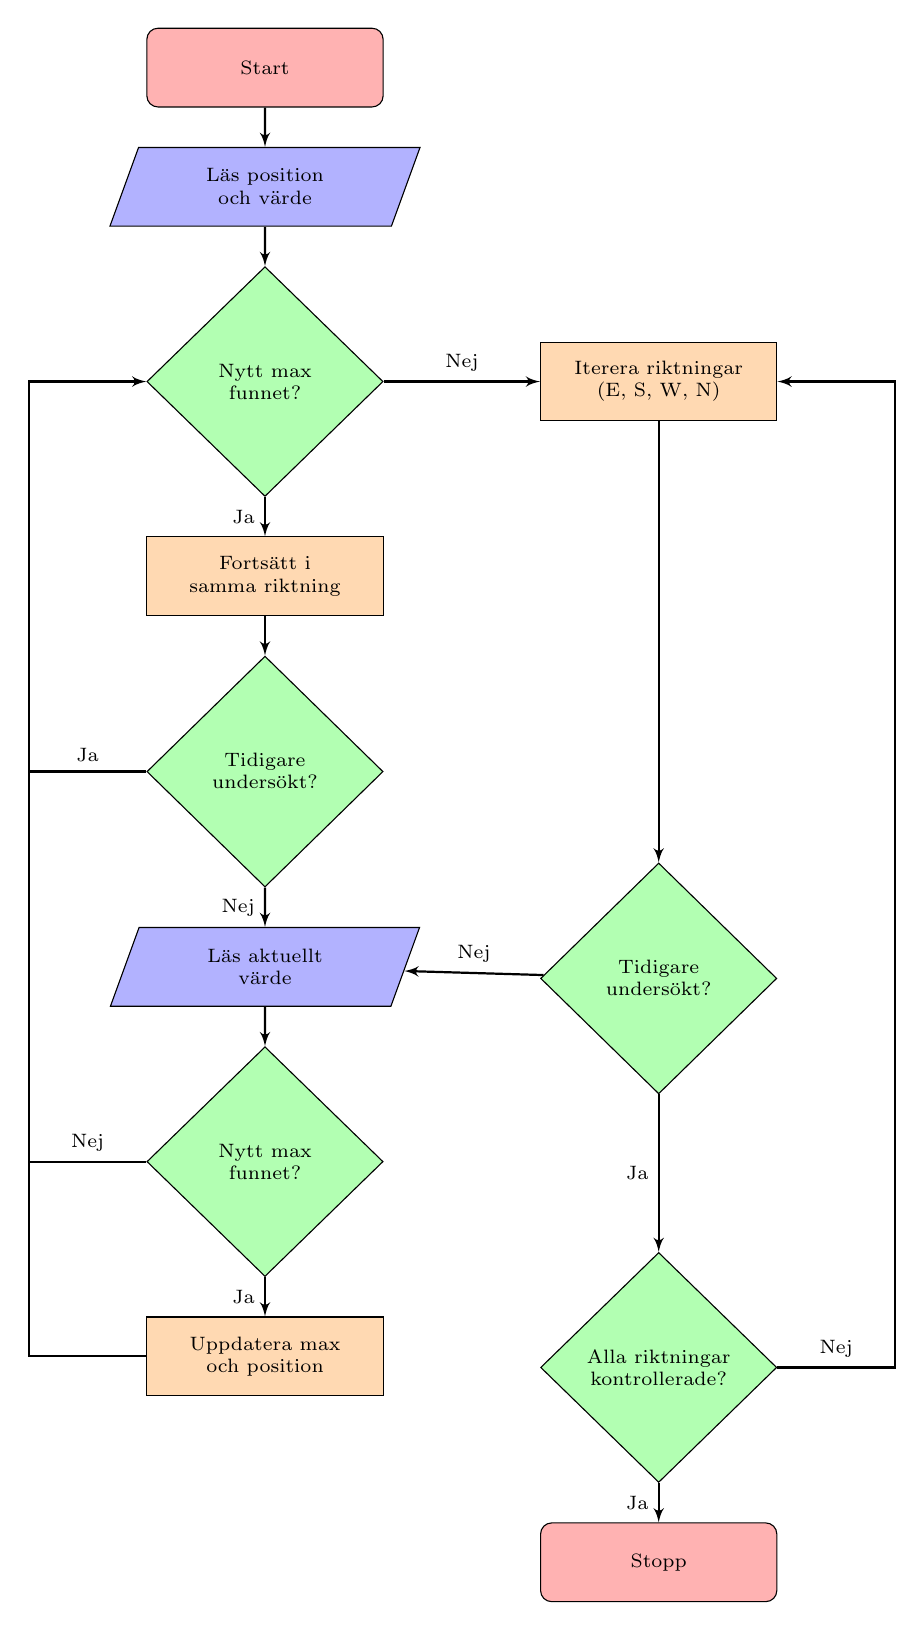
\begin{tikzpicture}[node distance=2cm]
    \tikzstyle{every node}=[font=\scriptsize]
    \node (start) [startstop] {Start};
    \node (inp1) [io, below=5mm of start, text width=20mm] {Läs position och värde};
    \node (success) [decision, below=5mm of inp1, text width=20mm] {Nytt max funnet?};
    \node (iterate) [process, right of=success, text width=25mm, xshift=3cm] {Iterera riktningar (E, S, W, N)};
    \node (prev1) [decision, below=56mm of iterate, text width=20mm] {Tidigare undersökt?};
    \node (allprev) [decision, below=20mm of prev1, text width=20mm] {Alla riktningar kontrollerade?};
    \node (same) [process, below=5mm of success, text width=25mm] {Fortsätt i \hbox{samma} riktning};
    \node (prev2) [decision, below=5mm of same, text width=20mm] {Tidigare undersökt?};
    \node (inp2) [io, below=5mm of prev2, text width=20mm] {Läs \hbox{aktuellt} värde};
    \node (greater) [decision, below=5mm of inp2, text width=20mm] {Nytt max funnet?};
    \node (update) [process, below=5mm of greater, text width=25mm] {Uppdatera max och position};

    \node (stop) [startstop, below=5mm of allprev] {Stopp};

    \draw [arrow] (start) -- (inp1);
    \draw [arrow] (inp1) -- (success);
    \draw [arrow] (success) -- node[anchor=south] {Nej} (iterate);
    \draw [arrow] (success) -- node[anchor=east] {Ja} (same);
    \draw [arrow] (same) -- (prev2);
    \draw [arrow] (iterate) -- (prev1);
    \draw [arrow] (prev1) -- node[anchor=east] {Ja} (allprev);
    % \draw [arrow] (prev1) -- node[anchor=south] {Nej} +(-2.25,0) |- (inp2);
    \draw [arrow] (prev1) -- node[anchor=south] {Nej} (inp2);
    \draw [arrow] (allprev) -- node[anchor=east] {Ja} (stop);
    \draw [arrow] (allprev) -- node[anchor=south] {Nej} +(3,0) |- (iterate);
    \draw [arrow] (prev2) -- node[anchor=east] {Nej} (inp2);

    \draw [arrow] (inp2) -- (greater);

    \draw [arrow] (greater) -- node[anchor=east] {Ja} (update);

    \draw [draw, thick] (prev2) -- node[anchor=south] {Ja} +(-3,0);
    \draw [draw, thick] (greater) -- node[anchor=south] {Nej} +(-3,0);

    \draw [arrow] (update) -- +(-3,0) |- (success);

\end{tikzpicture}
% section sokalgoritm (end)
\end{document}